\documentclass{article}
\usepackage{gensymb}
\let\vec\mathbf
\usepackage{float}
\usepackage{graphicx}
\graphicspath{{./documents/}{./figs}}
\begin{document}
\begin{enumerate}
\item In the given figure, $ PQ $ is tangent to the circle centred at $ \vec{O} $. 
	If $ \angle{AOB}=95^{\degree} $, then the measure of $ \angle{ABQ} $ will be.
\begin{figure}[H]
\centering
	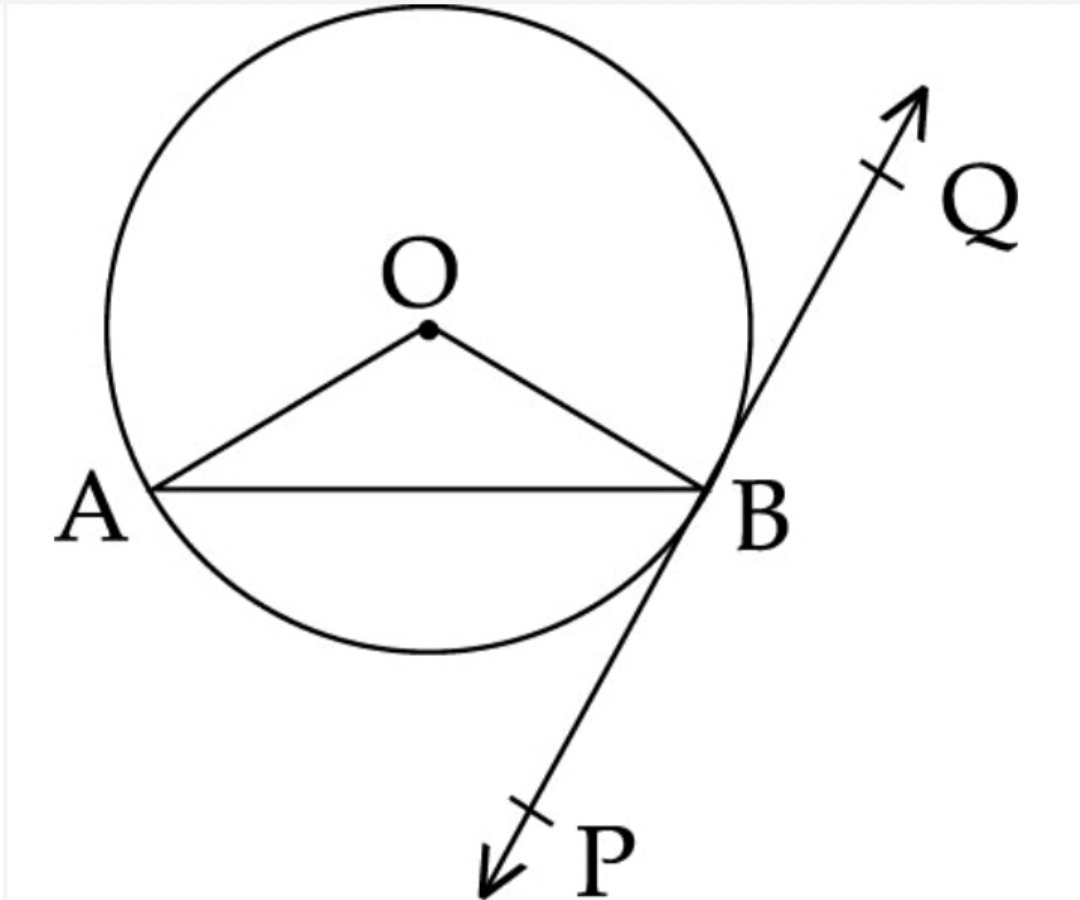
\includegraphics[width=\columnwidth]{fig1.jpg}
	\caption{}
	\label{fig}
\end{figure}
		\begin{enumerate}
			\item $ 47.5^{\degree} $
			\item $ 42.5^{\degree} $
			\item $ 85^{\degree} $
			\item $ 95^{\degree} $
		\end{enumerate}
	\item (a) Two tangents $ TP $ and $ TQ $ are drawn to a circle with center $ \vec{O} $ from an external 
		point $ \vec{T} $. prove that $ \angle{PTQ}=2\angle{OPQ} $.
		\begin{figure}[H]
			\centering
			\includegraphics[width=\columnwidth]{fig2.jpg}
			\caption{}
			\label{fig}
		\end{figure}
		(b) In the given figure, a circle is inscribed in a quadrilateral $ ABCD $ in which 
		$ \angle{B}=90^{\degree} $. If $ AD = 17 cm, AB = 20 cm $ and $ DS = 3 cm $, 
		then find the radius of circle.
		\begin{figure}[H]
			\centering
			\includegraphics[width=\columnwidth]{fig3.jpg}
			\caption{}
			\label{fig}
		\end{figure}
	\item The discus throw is an event in which an atlete attempts to throw a discus. The athlete spins anti-
		clockwise around one and a half times through a circle,Then the throw. When released, 
		The discus travels along the tangent to the circular spin orbit.
		\begin{figure}[H]
			\centering
			\includegraphics[width=\columnwidth]{fig4.jpg}
		\end{figure}
		In the given figure, $ AB $ is one such tangent to a circle of radius 75 cm. Point $ \vec{O} $
		is center of the circle and $ \angle{AOB}=30^{\degree} $. $ PQ $ is parallel to $ OA $.
		\begin{figure}[H]
			\centering
			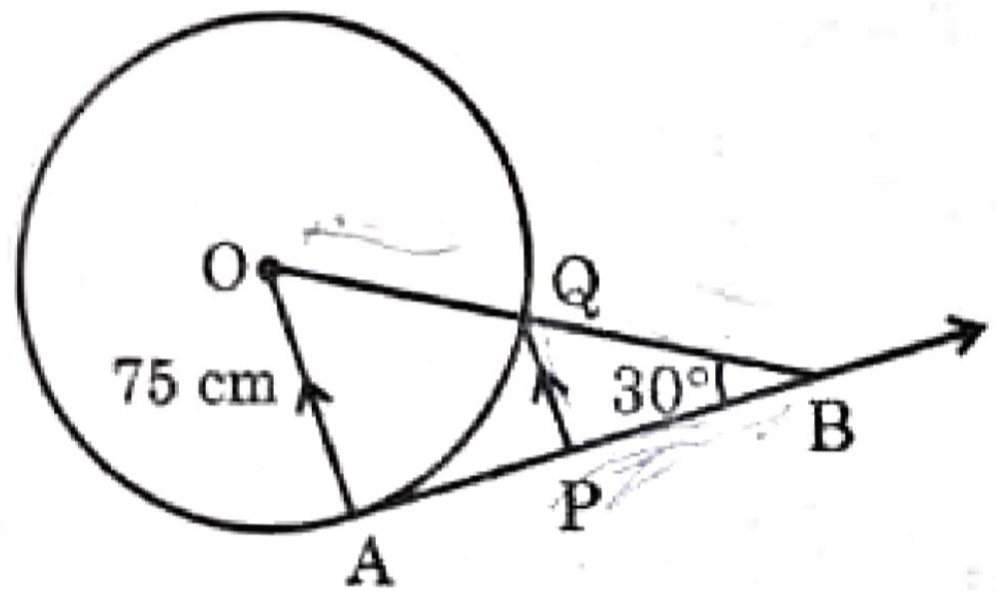
\includegraphics[width=\columnwidth]{fig5.jpg}
			\caption{}
		        \label{fig}
		\end{figure}
		Based on above information :
		\begin{enumerate}
			\item find the length of $ AB $.
			\item find the length of $ OB $.
			\item find the length of $ PQ $.
		\end{enumerate}
	\item In the given figure, The quadrilateral $ PQRS $ cirumscribes a circle. Here $ PA+CS $ is equal to :
		\begin{figure}[H]
			\centering
			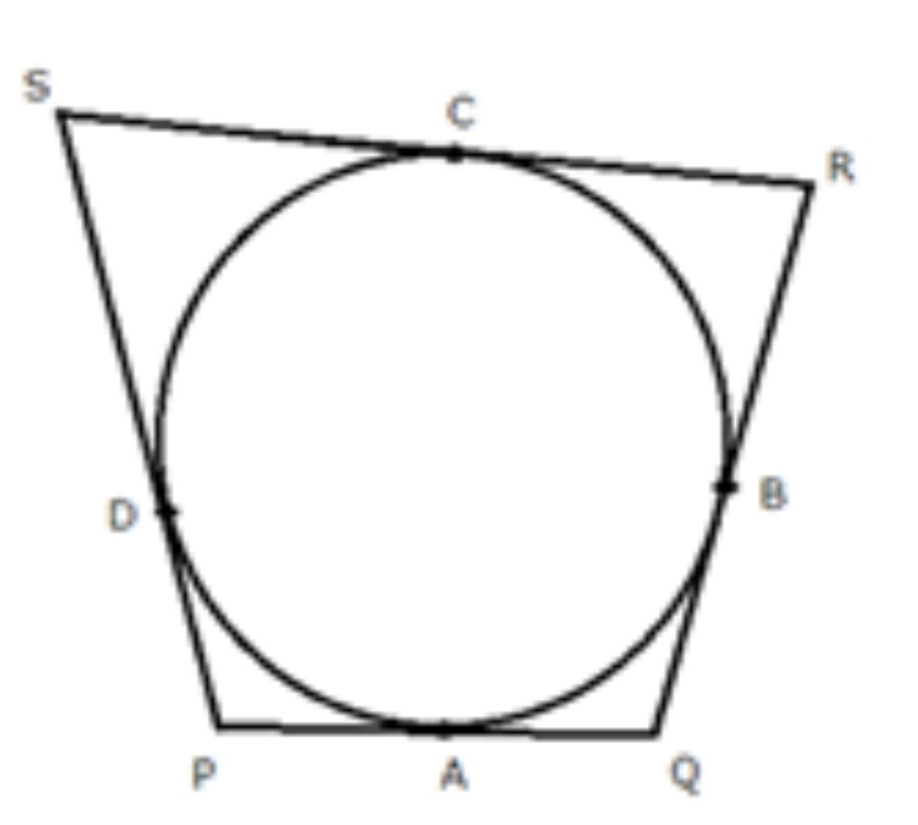
\includegraphics[width=\columnwidth]{fig6.jpg}
			\caption{}
			\label{fig}
		\end{figure}
		\begin{enumerate}
			\item $ QR $
			\item $ PS $
			\item $ PR $
			\item $ PQ $
		\end{enumerate}
	\item In the given figure, $ \vec{O} $ is the center of the circle. $ AB $ and $ AC $ are tangents drawn 
		to the circle from point $ \vec{A} $. If $ \angle{BAC}=65{\degree} $, Then find the measure of 
		$ \angle{BOC} $.
		\begin{figure}[H]
			\centering
			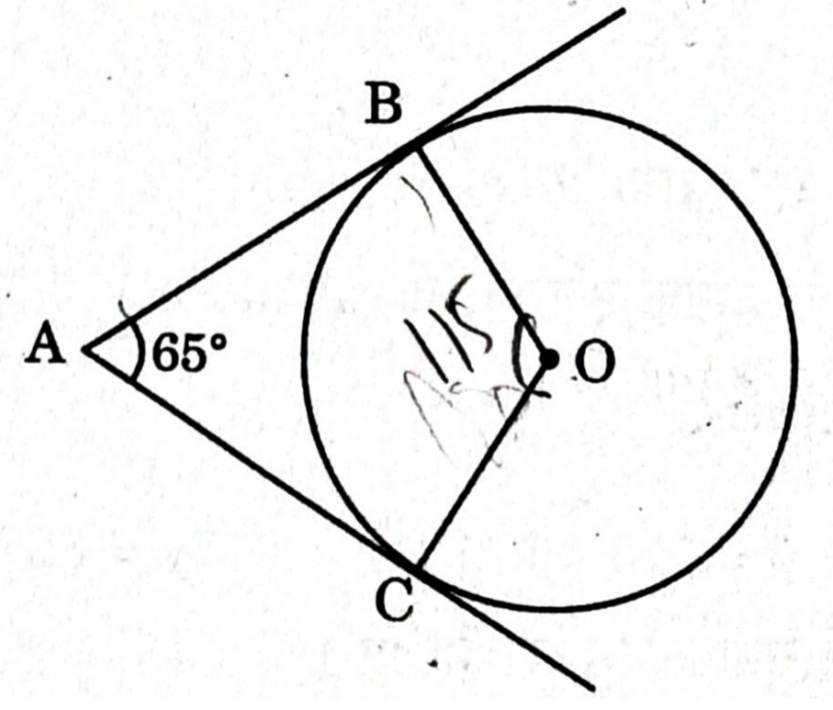
\includegraphics[width=\columnwidth]{fig7.jpg}
			\caption{}
			\label{fig}
		\end{figure}
	\item In the given figure, $ \vec{O} $ is the center of the circle and BCD is a tangent to it at
		$ \vec{p} $. Prove that $ \angle{BAC}+\angle{ACD}=90^{\degree} $\\
		\begin{figure}[H]
              \centering          
        	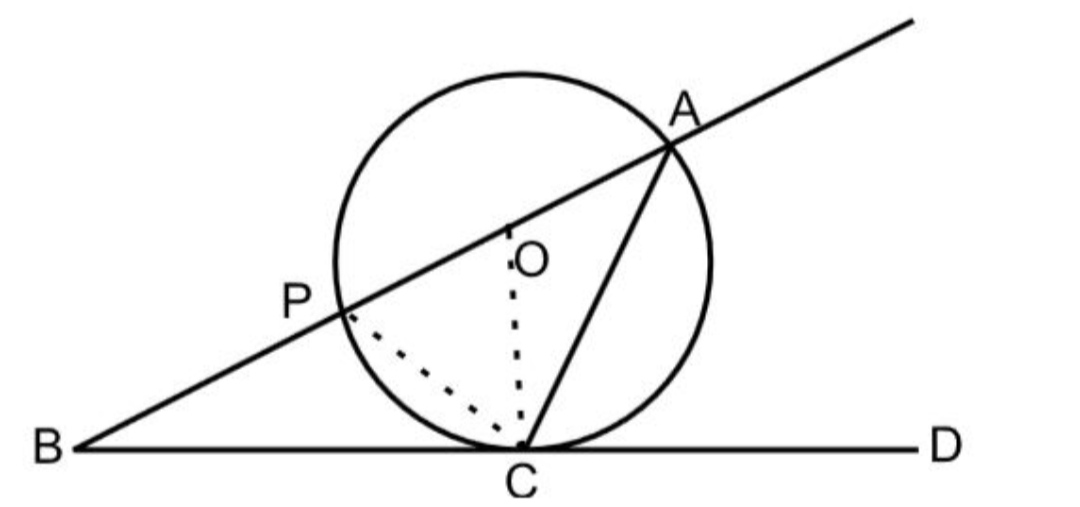
\includegraphics[width=\columnwidth]{fig8.jpg}     
                        \caption{}  
                        \label{fig}
		\end{figure}
	\item In the given figure, $ PT $ is a tangent to the circle with center $\vec{O}$. If $ \angle{TPO}=
		25^{\degree} $, Then x is equal to :
		\begin{figure}[H]
			\centering
			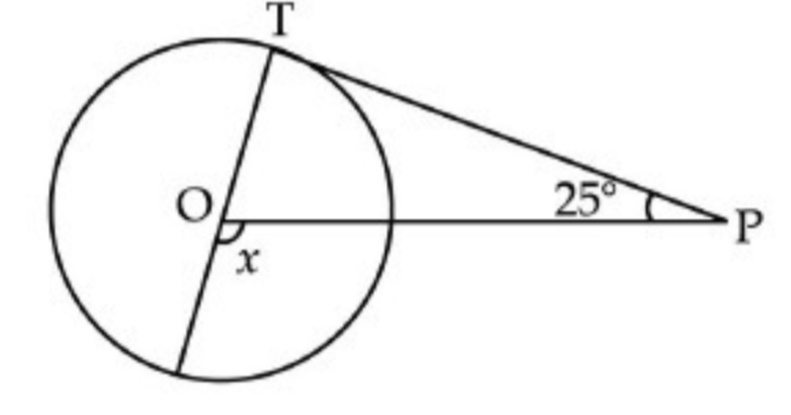
\includegraphics[width=\columnwidth]{fig9.jpg}
			\caption{}
			\label{fig}
		\end{figure}
		\begin{enumerate}
			\item $ 25^{\degree} $
			\item $ 65^{\degree} $
			\item $ 90^{\degree} $
			\item $ 115^{\degree} $
		\end{enumerate}
	\item In the given, $ TA $ is a tangent to the circle with center $ \vec{O} $ such that $ OT = 4 cm $, 
		$ \angle{OTA}=30{\degree} $, Then length of TA is :
		\begin{figure}[H]
			\centering
			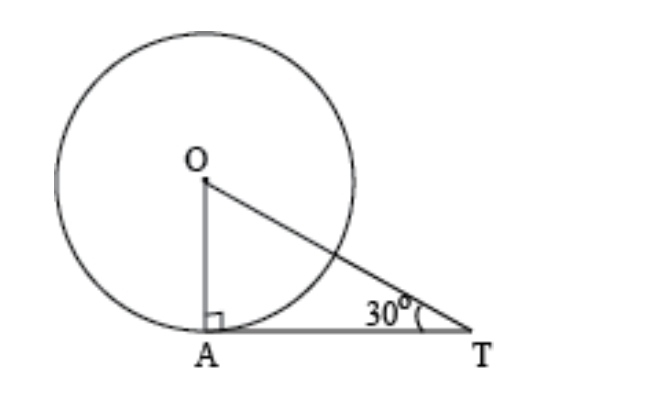
\includegraphics[width=\columnwidth]{fig10.jpg}
			\caption{}
			\label{fig}
		\end{figure}
		\begin{enumerate}
			\item 2 $ \sqrt{3} $ cm
			\item $ 2 cm $ 
			\item 2 $ \sqrt{2} $ cm
			\item $ \sqrt{3} $ cm
		\end{enumerate}
	\item Two concentric circles are of radii 5 cm and 3 cm. Find the length of he chord of the larger circle 
		which touches the smaller circle.






	
\end{enumerate}
\end{document}
